\section{System Models}
	This paper considers a robotic computation system consisting of a set of computation tasks and limited computation resources such as CPU cores. 
    The primary objective is to allocate resources effectively to optimize system performance in dynamic environments.
    This section introduces the system models, following notations from the real-time systems community~\cite{Buttazzo2011HardRC}.
    Frequently used notations are summarized in Table~\ref{notation_table}, while others are defined in context.
    % We use subscript to denote the \ith{i} instance of a vector. For example, $c_k$ denotes the \ith{k} element of vector $c$.

\begin{table}[]
\centering
\caption{Frequently-Used Notations}
\begin{tabular}{@{}ll@{}}
\toprule
Variables                                                             & Symbols         \\ \midrule
\ith{i} Computation task                                          & $\tau_i$        \\
Execution Time Distribution of $\tau_i$                                           & $\extDist{i}$           \\
Single Execution Time Value                                           & $c_i$           \\
Period                                                                & $T_i$           \\
Deadline                                                              & $D_i$           \\
Priority                                                              & $P_i$           \\
\begin{tabular}[c]{@{}l@{}}Response Time Probability Distribution of $\tau_i$  \end{tabular} & $\rtDist{i}$           \\
Scalar Response Time Value                                                         & $r_i$   \\
Task's configuration                                                  & $\lambda_i$     \\
Task's deadline miss threshold                                        & $\Theta_i$      \\
Task's importance                                                     & $w_i$           \\  \midrule
Scheduling Algorithm                                                  & $\mathcal{A}$   \\
\begin{tabular}[c]{@{}l@{}}Environment   vector\end{tabular}         & $\textbf{E}$           \\
$\tau_i$'s execution time distribution prediction function & $\mathcal{F}_i(\textbf{E}) \rightarrow \extDist{i} $ \\
Safety-Performance metric                                                             & $\textbf{SP}$   \\
Performance Metric                                                    & $\mathcal{P}()$ \\
Safety Metric                                                         & $\mathcal{S}()$ \\
Probability of an event                                                    & $\text{Pr}(event)$ \\
Probability Distribution & $\mathcal{D}$ \\
\\\bottomrule
\end{tabular}
\label{notation_table}
\end{table}
	
	
	\subsection{Computation Tasks}
    \label{section: system_model_tasks}
    A computation task represents an independent high-level application, such as motion planning or obstacle detection.
    For simplicity of presentation, we assume each task uses one CPU core each time.
    How to optimize other types of tasks models is discussed in Section~\ref{section: gang}.

	
	Most robotic tasks are modeled as periodic tasks\footnote{Tasks with non-constant periods, called sporadic tasks, have a minimum arrival interval between successive executions. These sporadic tasks are often treated as periodic tasks during schedulability analysis to simplify the modeling process} $\tau$. 
    We use $\boldsymbol{\tau}$ to denote the task set under consideration, $\tau_i$ to denote the \ith{i} task.
    Each task $\tau_i$ is characterized by five parameters: probability distribution of execution time $\extDist{i}$, period $T_i$, deadline $D_i$, and its run-time configurations $\lambda_i$:
	\begin{equation}
		\tau_i: [\extDist{i}, T_i, D_i, \lambda_i] 
		\label{eq_notation_task}
	\end{equation}
	
	
	\begin{definition}[Execution time, $\extDist{i}$]
		A task's execution time is a probability distribution of the time needed by one standard processor\footnote{Different processors may have different speed. A standard processor in this context means that the execution time is measured on a processor whose speed is normalized.} to finish its execution without interruption.
	\end{definition}
    The task's execution time is modeled as a probability distribution~\cite{Maxim2013ResponseTA}, reflecting variability due to factors like input data, operating system (OS) behavior, and hardware performance.
    This approach captures uncertainty while avoiding pessimistic worst-case assumptions.
    In experiments, due to the stringent need to maintain low scheduling overhead, we assume the execution time follows Gaussian distribution to reduce the optimization cost.

	
	\begin{definition}[Period, $T_i$]
		A task $\tau_i$ releases one job\footnote{According to Buttazzo~\cite{Buttazzo2011HardRC}, ``Periodic tasks consist of an infinite sequence of identical activities, called instances or \textit{jobs}, that are regularly activated at a constant rate.''} J for execution every $T_i$ time units.
	\end{definition}
    In other words, the periodic task $\tau_i$ needs to be run for one time every $T_i$ time units.
	
	\begin{definition}[Deadline, $D_i$]
		Deadline $D_i$ refers to the maximum amount of time that a job must be completed to avoid causing potential damage to the system.
	\end{definition}
	
	% The deadline definition above is the same as the \textit{relative deadline} used in the real-time system community. 
    In most cases, the deadline $D_i$ is assumed to be no larger than the period $T_i$~\cite{Buttazzo2011HardRC, Wang2023RTAS}.
	
	
	\begin{definition}[Task configurations, $\lambda_i$]
		\label{def_task_config}
		A task $\tau_i$'s configuration $\lambda_i$ includes the parameters that influence the tasks' execution time distribution and output quality.
	\end{definition}
	
	For example, some tasks such as motion planning may adopt a searching-based algorithm, which often takes the running time limits as one configuration parameter.
	The running time limits influence both the execution time distribution and the task's output quality (longer time limits mean higher output quality).
	In this paper, we focus on the running time limit because it is related to both the performance and safety of a task.
	However, other parameters can be incorporated into our framework in a similar way.
	
	
\begin{figure*}[htbp]
\centering
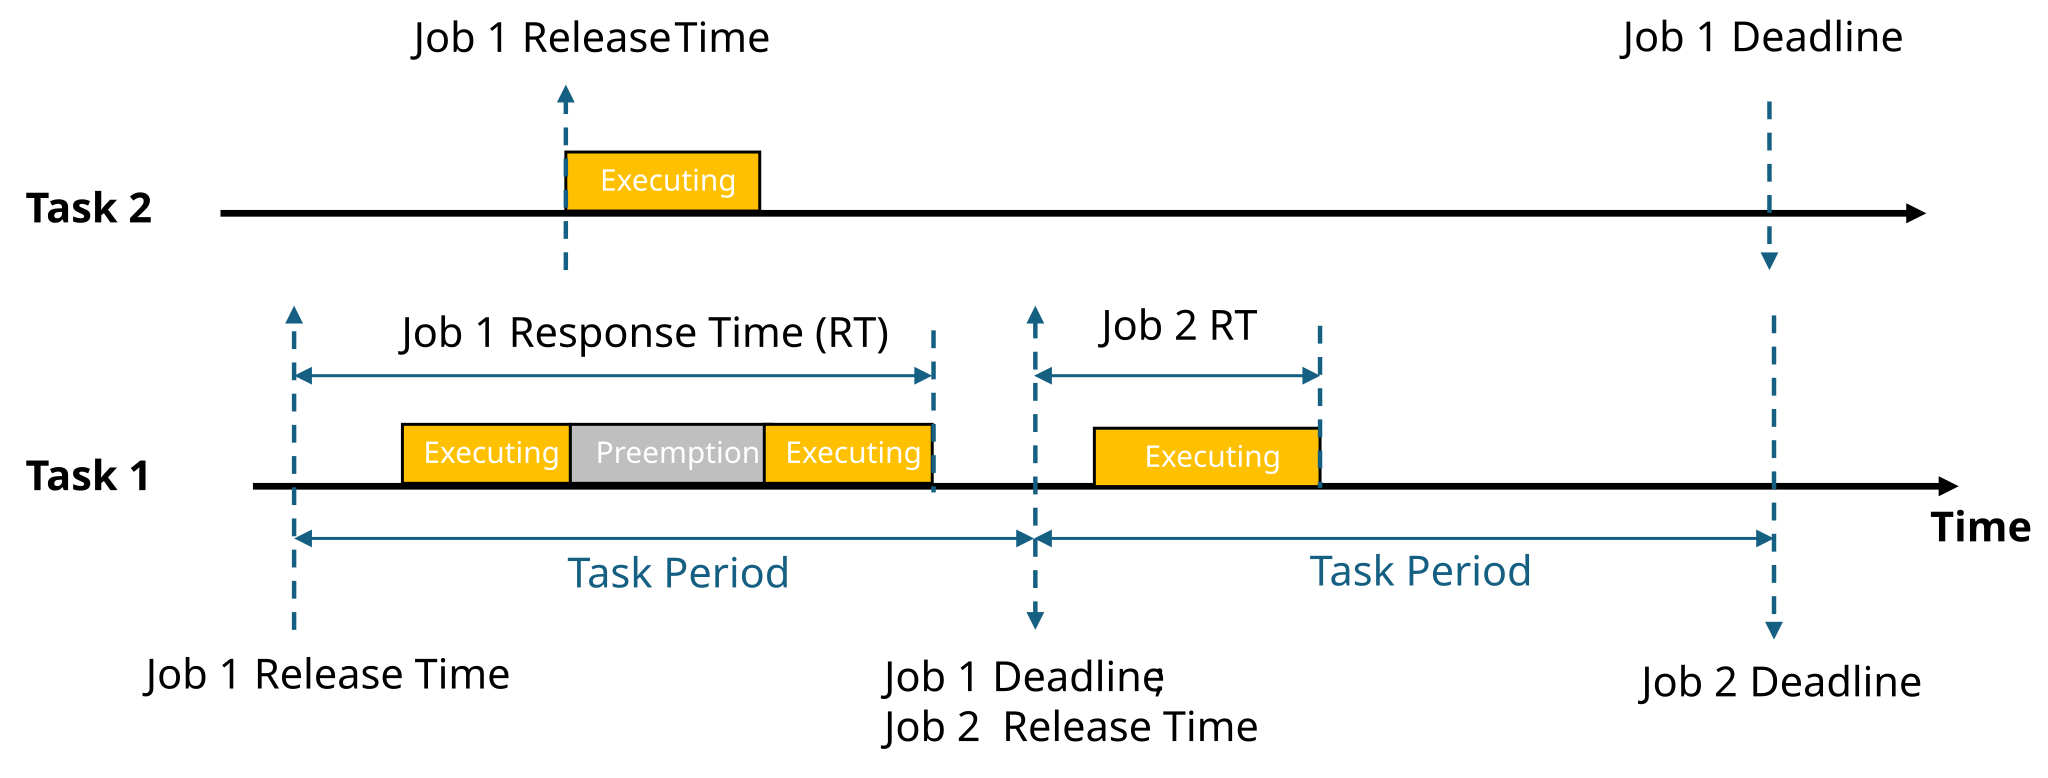
\includegraphics[width=0.8\textwidth]{pictures/RTS_concepts.pdf}
\caption{Concepts adopted from the Real-Time Systems Area. The figure above shows two tasks' scheduling, where task 2 has higher priority than task 1 and both are scheduled to run on the same CPU core. When task 2 releases a job to execute, it preempts task 1's job. The job 1 of task 1 continues execution after task 2's job 1 finishes execution.
}
\label{fig_rts_concepts}
\end{figure*}
    
	
	\subsection{Computation Platform}
	\label{section_rta_distribution}
    This paper adopts a computation platform that is common in practice and the literature~\cite{Ash23RAL, Wang2023OptimizingLET, Verucchi2020LatencyAwareGO}.
	The computation platform is modelled as a multi-core system where each task is assigned to a known core using partitioned scheduling~\cite{Buttazzo2011HardRC}.
	Disabling task migration reduces scheduling overheads and provides more predictable response time~\cite{Brandenburg2016GlobalSN}.
    Each task is assigned a unique priority $P_i$, which could change from time to time based on scheduling algorithms.
    Under preemptive scheduling, higher-priority tasks could preempt lower-priority tasks when high-priority tasks become ready, which are paused and resumed later.
    In this paper, we focus on soft real-time systems, where tasks that miss deadlines by small margins can still contribute to system functionality.
	
	We use priority assignments to describe the relative importance of tasks:
	\begin{definition}[Priority Assignments, $\mathcal{A}$]
		A priority assignment vector for a task set $\boldsymbol{\tau}$ is a complete ordered sequence of tasks $\boldsymbol{\tau}$, where higher-priority tasks appear earlier.
	\end{definition}
    
    In most operating systems such as Linux, the priority assignment needs to be converted into priority values to be useful, see more in Section~\ref{section_pa_values}.
	
	\subsection{Schedulability Analysis}
	\label{sectino_schedulability_analysis}

    \textit{Schedulability} determines whether all tasks can meet their deadlines under a given scheduling algorithm.
    There are two types of schedulability: \textit{Hard} Schedulability, where all tasks must always finish before their deadlines;
    \textit{Soft} Schedulability, where the probability of any task missing its deadline is below a given threshold (some papers may use a slightly different definition).
    This paper focuses on soft schedulability because it is not only more general than hard schedulability, but also more practical for robotic systems and balances resource constraints with system performance.
    
	
	Response time analysis is one of the most well-studied methods to analyze schedulability:
	\begin{definition}[Response time $r_i$]
		A task $\tau_i$'s response time $r_i$ includes its execution time $\extDist{i}$ and the time that it waits to obtain the required computation resources (\eg being preempted).
	\end{definition}
	Considering the random nature of execution, analyzing the probability distribution of response time is more reliable:
	\begin{definition}[Response time distribution $\rtDist{i}$]
		A task $\tau_i$'s response time distribution $\rtDist{i} = \{r_i^{(k)}: p_i^{(k)}\}$ is a discrete probability distribution of $k$ items, where each item describes that the probability of having response time as $r_i^{(k)}$ is $p_i^{(k)}$.
	\end{definition}
    
	Response time distribution can be obtained either experimentally or analytically. The analytical methods are much faster and simpler than the experimental methods but are also more pessimistic. Section~\ref{section_rta} introduces the two analytical methods.
	
	